\chapter{轨迹跟踪}
\section{基础理论知识}
\subsection{L1轨迹跟踪}
本节主要参考文献\href{attachment/A New Nonlinear Guidance Logic for Trajectory Tracking 6.2004-4900.pdf}{\texttt{A New Nonlinear Guidance Logic for Trajectory Tracking}}。

L1轨迹跟踪控制算法的核心包括两个部分:\\
(1)在期望轨迹上寻找与飞机相距 L1 的参考点,并计算速度矢量与目标向量间夹角$\eta$\\
(2)计算侧向加速度指令为:
\begin{equation}
    a_{s_\rm{cmd}} = 2 \frac {V^2}{L_1} \sin\eta
\end{equation}
\begin{figure}[htbp]
	\figskip
	\centering
	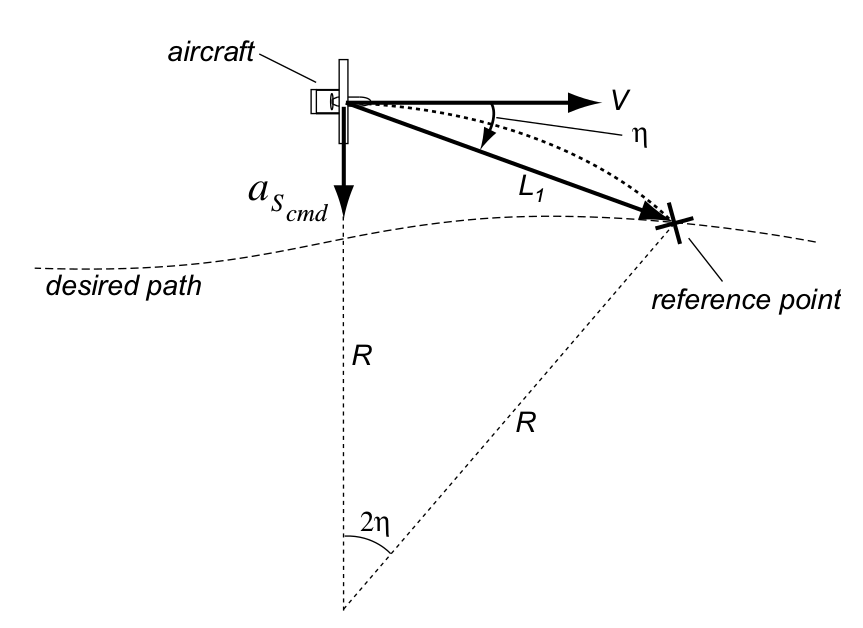
\includegraphics[width = 0.7\textwidth,trim = 0 -0 0 -0,clip]{L1.png}	  
	\caption{\label{fig: L1} L1轨迹跟踪计算示意图}
\end{figure}

通常轨迹跟踪都会针对直线轨迹和定点盘旋轨迹分别讨论。在直线轨迹跟踪中,侧偏距误差$d$可以用飞机质心与期望航线的垂直距离表示;在定点盘旋轨迹跟踪中,侧偏距误差$d$用飞机质心与圆的距离表示(质心到圆心距离 - 圆半径)。所以在应用L1轨迹跟踪算法时,需要考虑$d>L_1$的情况,也就是飞机距离轨迹较远的情况。

对于直线轨迹跟踪,在图\ref{fig: L1-line}中,可以对$\eta_1$进行限制,如$-30^\circ \le \rm{sat}(\eta_1) \le 30^\circ$。而对于盘旋轨迹,可以在$d>L_1$时先进行直线轨迹跟踪,期望直线可以取为过质心的圆切线(圆半径可适当增加一个差值),在$d<L_1$后再转入盘旋跟踪。另外在定点盘旋跟踪中需要利用速度向量与心心距向量判断旋转的方向(滚转的正负号)。

\begin{figure}[htbp]
	\figskip 
	\centering
	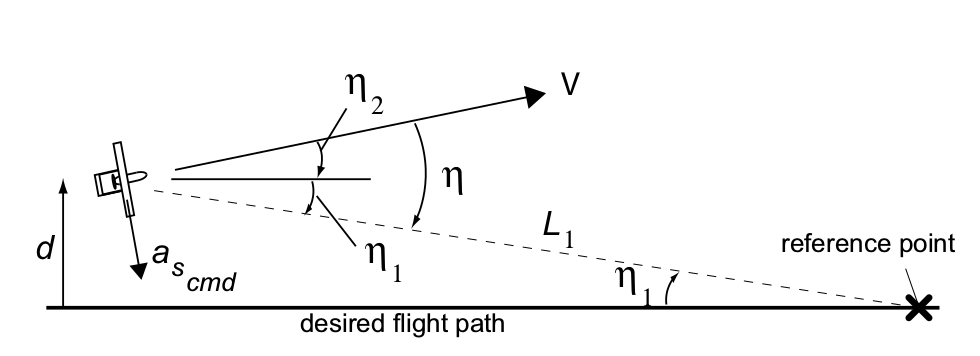
\includegraphics[width = 0.7\textwidth,trim = 0 -0 0 -0,clip]{L1-line.png}	  
	\caption{\label{fig: L1-line} 直线轨迹中L1轨迹跟踪计算示意图}
\end{figure}

在\href{attachment/L1t.m}{Matlab仿真}中验证定点盘旋算法时,通过几何关系可以直接计算$\eta$角度,再按原始公式计算加速度指令。而论文中则采用$\frac{V^2}{R} - \ddot{d}$进行近似,其中$\ddot{d}$在实现时似乎不方便计算。计算$\eta$角度时,涉及相交圆的求解,\href{http://blog.csdn.net/zx3517288/article/details/53326420}{参考这里的推导}。

最后,在L1算法中,给出了期望的加速度指令,如果假设飞机在进行高度不变的稳定盘旋时,侧向加速度指令等价于滚转角指令。而对于航向指令,论文中并没有提及,但是从PX4源码中可以看出,{\sout{直线轨迹时航向指令指向L1跟踪点,盘旋轨迹时航向指令始终指向圆心点}}两种轨迹下虽然给出了偏航指令,但在内环均保持协调转弯的偏航控制策略,而未跟踪该偏航角。
 
\subsection{进一步讨论}
以下讨论只针对固定翼,且假设1具有高度保持系统,2内环姿态控制的偏航通道按照协调转弯方式进行控制。多旋翼在做轨迹跟踪时,需要独立给出航向跟踪指令。

首先考虑偏盘旋轨迹跟踪问题,对于给定的飞行速度$V_a$和侧向加速度$a_s$(等价滚转角),在稳定盘旋时盘旋半径为$R = V_a^2 / a_s$。显然对于给定的盘旋半径,可以计算盘旋时的侧向加速度。如果以跟踪盘旋轨迹的圆心点作为参考点,那么无人机相对该参考点的运动可以分解为两部分:1.质心与圆心连线上的运动;2.相对圆心的圆周运动。若以侧向加速度为控制量,那么有

\begin{equation}
    a_{s_\rm{cmd}} = a_{\parallel} + a_{\perp} = \rm{f}(d,V_a) + \frac{V_a^2}{R}
\end{equation}
其中,$d$表示侧向轨迹偏差,$\rm{f}(d,V_a)$表示侧向偏差及飞行速度的函数,可以理解为对$d$的PD控制律。一种更形象的解释为:$a_{\perp}$能够让无人机产生一个指定半径的圆轨迹,$a_{\parallel}$能够让这个圆轨迹的圆心逐渐移动到指定的位置上。

\begin{figure}[htbp]
	\begin{minipage}[t]{0.5\textwidth}
	\centering
	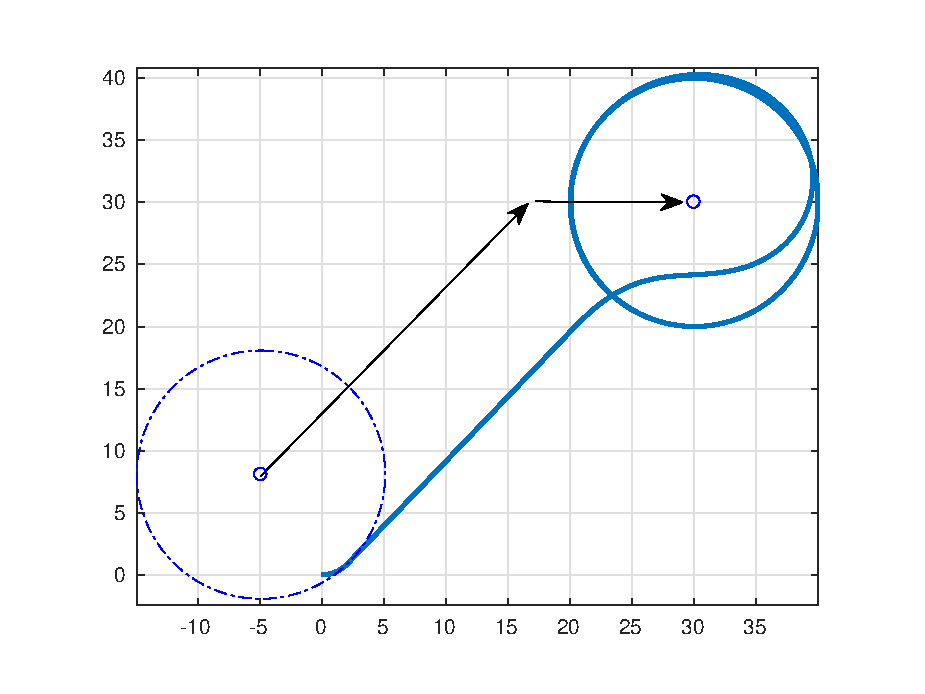
\includegraphics[width = 0.9\textwidth]{path1.eps}
	\caption{\label{fig: path1} 一种更形象的解释轨迹跟踪}
	\end{minipage}
	\begin{minipage}[t]{0.5\textwidth}
	\centering
	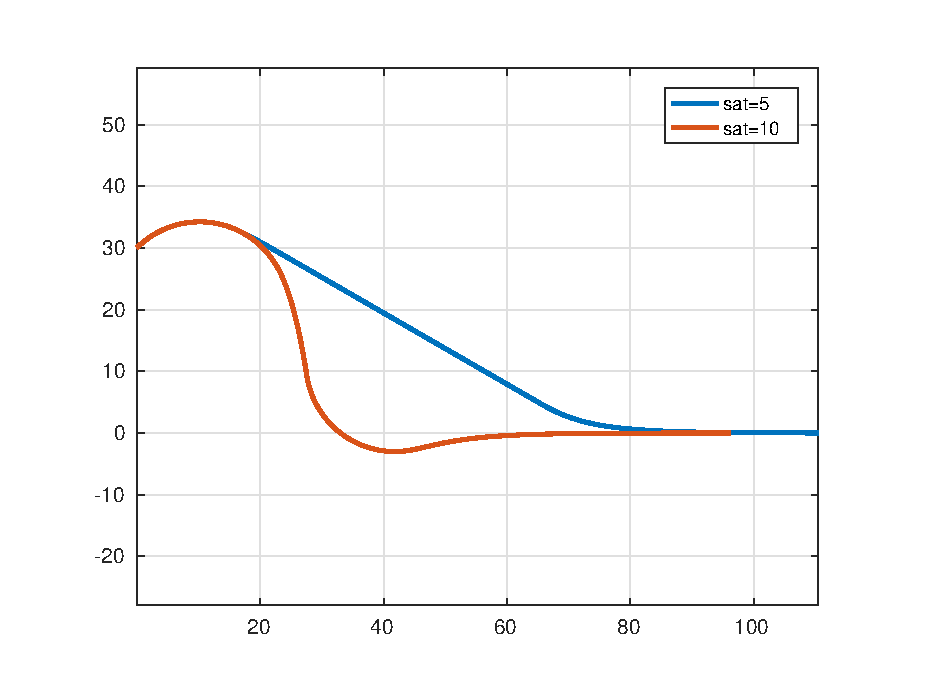
\includegraphics[width = 0.9\textwidth]{path2.eps}
	\caption{\label{fig: path2} 直线轨迹跟踪,对$d$取不同约束值的轨迹}
	\end{minipage}
\end{figure}


对于直线轨迹跟踪,可以认为是半径为$\infty$的圆轨迹,求解算法基本一致,只是需要在计算时限制$\rm{f}(d,V_a)$中的$d$值,以保证飞机能始终向前飞行,而不会对着航线飞行。

\subsection{其他的几种轨迹跟踪}
本节主要参考文献\href{attachment/Unmanned Aerial Vehicle Path Following.pdf}{\texttt{Unmanned Aerial Vehicle Path Following}}。


\section{MPC控制及动态路径跟踪}
模型预测控制(MPC)可以用于外环的路径跟踪控制上。若假设纵向控制中已经设计好了速度、高度控制器(比如TECS),且假设偏航控制能够按照协调转弯的方式保持飞机无侧滑,那么二维路径跟踪问题就可以转换成以侧向加速度/滚转角为输入量、以姿态闭环为被控系统的SISO控制问题。若内环控制器具有较好的控制性能,那么姿态闭环可以动态线性化为一个二阶串级线性系统,这时可以应用MPC进行控制。

MPC的核心问题就是在于对优化目标函数的设计及求解,若以师姐论文中的动态路径跟踪(避障)问题为例,优化目标函数可以设计为
\begin{equation*}
	J = \sum_i^N J^{(i)} = \sum_i^N \left(J_{path}^{(i)} + J_{angle}^{(i)} + J_{obs}^{(i)} + J_{final}^{(i)} \right)
\end{equation*}
其中,$N$为滚动优化的长度,$J^{(i)}$为滚动优化中每一步的罚函数,$J_{path}^{(i)}$为路径跟踪误差,$J_{angle}^{(i)}$飞行航向跟踪误差,$J_{obs}^{(i)}$为避障罚函数 + $J_{final}^{(i)}$为终点吸引罚函数。具体代码在\href{attachment/mympc.m}{\texttt{这里}}。运行的结果为:

\begin{figure}[htbp]
	\figskip 
	\centering
	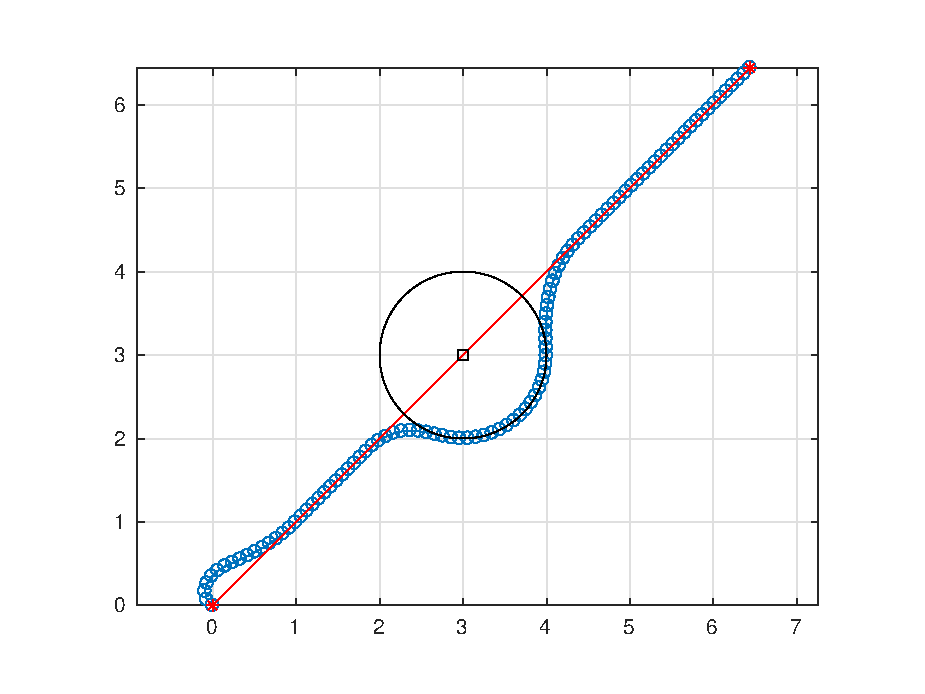
\includegraphics[width = 0.7\textwidth,trim = 0 -0 0 -0,clip]{mpc.eps}	  
	\caption{\label{fig: mpc} 一个简单的基于MPC的动态路径跟踪}
\end{figure}



